\chapter{Computing in DUNE}
\label{ch:exec-comp}

%\textit{
This chapter briefly describes the \dword{dune} computing model, which touches on all elements of the \dword{dune} \dwords{nd} and \dwords{fd} and their physics programs.  More detailed aspects of the model may be found in Appendix~\ref{appx:es-comp} of this \dword{tdr} volume.  \dword{dune} will produce a complete technical design report for computing over the next two years.%}

%\fixme{Should this paragraph be in italics? To be consistent with the rest of the document, I suggest it should be in non-italic text.}
% HMS no idea who made this italics. 

%%%%%%%%%%%%%%%%%%%%%%%%%%%%%%%%%%%%%%%%
\section{Executive Summary}
\label{ch:exec-comp-es}

%\newdword{nersc}{NERSC}{National Energy Research Computing Facility at \dword{lbnl}}

The \dword{dune} experiment will commission the first \nominalmodsize fiducial mass \dword{lartpc} module between 2024 and 2026 with a long data-taking run, and the number of modules will increase to four between 2026 and 2036.  An active prototyping program is in place with  a short test beam run in 2018 at \dword{cern}.  These tests used  a \SI{700}{t}, 15,360 channel prototype \dword{tpc} with \dword{sp} readout.  Tests of a \dword{dp} detector of similar size are scheduled for mid-2019.   The \dword{dune} experiment has already  benefited greatly from these initial tests.  The collaboration has recently formed a formal \dword{csc}, with significant participation of European institutions and interest from groups in Asia, to develop common software and computing and formalize resource contributions.

The consortium resource model benefits from the existing \dword{osg}  and \dword{wlcg} infrastructure developed for the \dword{lhc} and broader \dword{hep} community.  \dword{dune} is already using global resources to simulate and analyze  \dword{pdsp} data.  Several European institutions are part of this resource pool, making significant contributions to the \dword{pdsp} and \dword{pddp} programs.  We expect this global computing consortium to grow and evolve as we begin gathering data from the full \dword{dune} detector in the 2020s.

The long-term \dword{dune} science program should produce volumes of raw data similar in scale to the data volumes that current \dword{lhc} Run-2 experiments have already successfully handled.  Baseline predictions for the \dword{dune} data, depending on actual detector performance and noise levels, are $\sim\,$\SI{30}{PB} of raw data per year.  These data, with simulations and derived analysis samples, must be available to all collaborating institutions.  We anticipate that institutions around the world will both contribute and use storage and CPU resources for \dword{dune}.

The \dword{dune} computing strategy starts with considerable infrastructure in place for international computing collaboration, in part thanks to the \dword{lhc} program.  Additional large non-\dword{lhc} experiments,  such as \dword{lsst}, the \dword{belleii} B-factory experiment, and \dword{dune}  will begin operation over the next decade and must use and expand upon this model to encourage international cooperation.  The broader \dword{hep} community is organizing common efforts through the \dword{hsf}~\cite{Alves:2017she}.  The \dword{hsf} is an organization of interested parties using the extensive knowledge gained over the past two decades to anticipate the needs of experiments over the next two decades, and to develop a sustainable computing landscape for the \dword{hep} community.  The \dword{hsf} white papers and roadmaps emphasize common tools and infrastructure as the foundation of this landscape.

The \dword{dune} computing strategy heavily leverages the \dword{hsf} model of common tools and infrastructure which feature data movement and storage, job control and monitoring, accounting, and authentication that both use and contribute to this global community.   \dword{dune} recognizes that other large-scale experiments have similar needs and will encounter complementary issues, thus driving worldwide cooperation on common tools as the most cost-effective way to fulfill the scientific missions of the experiments.  \dword{dune} pilot programs already use this model.  Most recently in data management and storage, \dword{fnal}, \dword{cern}, Rutherford Appleton Laboratory, and other academic institutions in the %United Kingdom ah
UK are collaborating on adapting and using the \dword{rucio} data management systems~\cite{Barisits:2019fyl}  to serve as the core data management system for \dword{dune}.

%Examples of 
This protoculture of international collaboration within \dword{dune} %were 
was demonstrated during the 2018 test beam run of the \dword{pdsp} detector  at \dword{cern}.  During this run, % the \dword{sp} ah
\dword{pdsp} produced raw data at rates of up to \SI{2}{GB/s}.  These data were transferred and stored in the archive facilities at \dword{cern} and \dword{fnal}, and replicated at sites in the UK and Czech Republic.  In a more recent commissioning test for the \dword{pddp} detector, similar data transmission rates %have been 
were achieved to \dword{cern}, \dword{fnal}, and the CCIN2P3 computer center in Lyon, France.

In total, \SI{1.8}{PB} of raw data were produced during the ten week test beam run, mimicking, within a factor of two, expected data rates and volumes from the initial running of the \dword{fd} complex.  The prototype run was used to examine and test the scalability of existing and proposed computing infrastructure and to establish operational experience within the institutions that have expressed interest in developing and constructing the \dword{dune} computing environment.  Our planning is primarily based on the measurements and information gained from the \dword{protodune} experience.  These measurements are proofs-of-concept for many of the systems, and their behavior can be reliably extrapolated to the projected levels needed for the complete \dword{dune} experiment. 

The \dword{protodune} experience highlights the significant technical challenges that must be overcome by 2024 for \dword{dune}. Among the most significant will be  1) the design of \dword{dune} specific systems able to integrate the large suite of ancillary data (e.g., configurations, calibrations, shower libraries) with the main \dword{tpc} datastream; 2) the potentially extreme size of some physics interactions, notably supernova bursts, that could produce data which overwhelm conventional processors; and 3) the continuing need for evolution of computing architectures and infrastructure over the next decade. These areas are unique to \dword{dune} where the limiting factor will be human effort. 

In summary, the \dword{dune} computing strategy must be global, working with partners worldwide, and collaborative because many of the computational challenges we face are also %those facing ah
faced by other, similar experiments.  We are extremely fortunate to have the \dword{protodune} experience and test data to exercise our computing infrastructure and develop algorithms for full \dword{dune} operations, although we know significant and interesting challenges lie ahead. 
 
%%%%%%%%%%%%%%%%%%%%%%%%%%%%%%%%%%%%%%%%
\section{Computing Consortium}
\subsection{Overview}
\label{ch:exec-comp-ovr}

The mission of the \dword{dune} %computing consortium (CSC) ah
\dword{csc} is to acquire, process, and analyze both detector data and  simulations for the %\dword{dune} ah
collaboration.  This mission must extend over all the primary physics drivers for the experiment and must do so both cost effectively and securely. The \dword{csc} provides the bridge between the online \dword{daq} and monitoring systems with the physics groups who develop high-level algorithms and analysis techniques to perform measurements using the  \dword{dune} data and simulations. The \dword{csc} works with collaborating institutions to identify and provide computational and storage resources.  %They provide ah
It provides the software and computing infrastructure in the form of analysis frameworks, data catalogs, data transport systems, database infrastructure, code distribution mechanisms, production systems, and other support services essential for recording and analyzing the data and simulations. 

The \dword{csc} works with national agencies and major laboratories to negotiate use and allocation of computing resources.  This work includes support for near-term R\&D efforts %like ah 
such as \dword{protodune} runs, and extends to designing, developing, and deploying the \dword{dune} computing model and its requisite systems. 
This includes evaluating major software infrastructure systems to determine their usefulness %for 
in meeting the \dword{dune} physics requirements.  These evaluations should identify opportunities to adopt or adapt existing technologies, and to engage in collaborative ventures with \dword{hep} experiments outside of \dword{dune}. 

%\fixme{this needs a different heading. AH  -- HMS don't understand this comment. The next paragraph is overview of the problem. }

At first glance,  the \dword{dune} CPU and storage needs %are ah
appear modest %on the scale of ah
compared to the corresponding needs for the high-luminosity \dword{lhc} experiments.  
However, the  beam structure, event sizes, and analysis methodologies make \dword{dune} very unlike collider experiments %in ah
in event processing needs and projected computational budgets. 
%\fixme{What are the features of these items that are different? AH} 
In particular, the large \dword{dune} event sizes (0.1-10 GB as opposed to 1-10 MB per detector readout) present a novel technical challenge when data processing and analysis are mapped onto  current and planned computing facilities. %\fixme{previous sentence needs clarification once we understand the novel aspects. AH} %In particular, the advent of high-performance computing systems optimized for parallel processing of large data arrays presents \dword{dune} with a potential advantage, as our event structure is more suited to those architectures than conventional tracker-based HEP data. AH
The advent of high-performance computing systems optimized for parallel processing of large data arrays is a great advantage for \dword{dune}. These architectures suit the uniform \dword{lar} \dword{tpc} raw data structure very well, in contrast to the more complex data structures and geometries present in conventional tracker-based \dword{hep} data. 
%\fixme{we need the background to understand why. AH}

%Neutrino oscillation analysis and parameter extraction also present %novel computational 
%challenges.  \fixme{what's novel about them? AH}

%These novel features of \dword{dune} data ah
\dword{dune} will require significant effort to adapt to emerging  %available 
global computing resources that % available to the experiment.ah 
%These global resources ah
  likely will be both more heterogeneous in computational capabilities (e.g., featuring CPU, GPU, and other advanced technologies) and more diverse in topological architectures and provisioning models.  The \dword{dune} \dword{csc} must %address these issues of diversity and architecture ah
be ready to fully exploit these global resources %available ah 
after 2026, allowing all collaborators to access the data and meet the scientific mission of the experiment.  

%%%%%%%%%%%%%%%%%%%%%%%%%%%%%%%%%%%%%%%%
\subsection{Resources and Governance}
\label{sec:exec-comp-res}

%The computing and software group is now a \dword{dune} consortium. ah
The \dword{csc} was formed from an earlier ad hoc \dword{dune} computing and software group. % in \fixme{date?}
The governance structure for the consortium is described in reference~\cite{bib:docdb12751}.  The consortium coordinates work across the collaboration, but funding comes from collaborating institutions, laboratories, and national funding agencies. %Aside from a small fraction of the consortium leadership, it is not supported by \dword{dune} or \dword{lbnf} project funds.  \fixme{lbnf?}

The %consortium 
\dword{csc} has an elected Consortium Lead %. The consortium leader 
who is responsible for subsystem deliverables and represents the consortium in the overall \dword{dune} collaboration.
In addition, technical leads act as overall project managers for the consortium. The technical leads report to the overall consortium leader.
\dword{csc} has both a host laboratory technical lead to coordinate between the \dword{dune} project and \fnal, which serves as the host laboratory, and an international technical lead to coordinate with other entities.
At least one of the three leadership roles should be held by a scientist from outside the US. 
Consortium management currently fills other roles by asking for volunteers.  A more formal structure for institutional contributions and commitments is under consideration. 

\begin{figure}[htp]
\centering
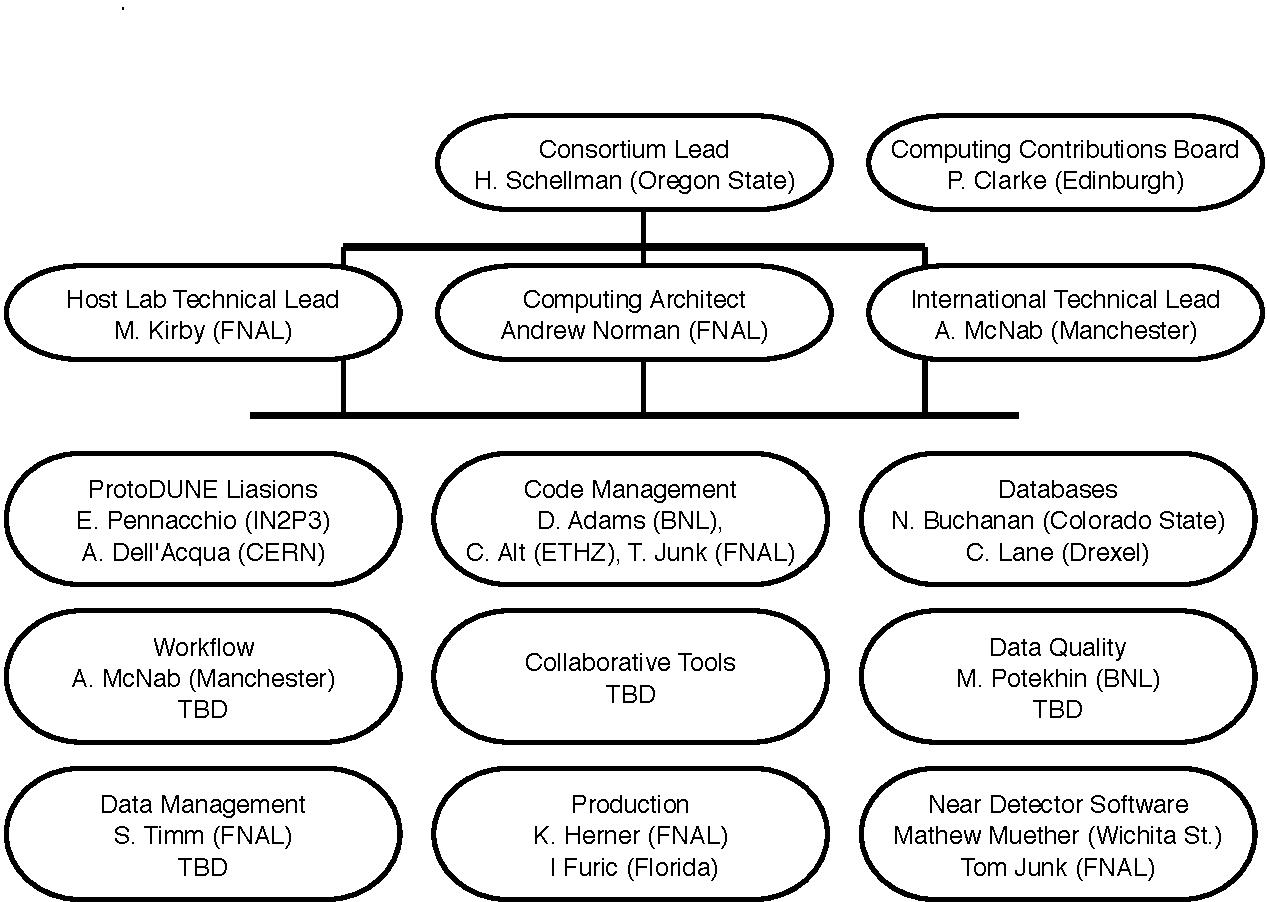
\includegraphics[height=4in]{graphics/comp-org-chart.pdf}
\caption[Organization chart for current \dshort{csc}]{Organization chart for current \dword{csc}. }
\label{fig:ch-exec-comp-org-es}
\end{figure}

\subsection{Scope of the Consortium}
\label{ch:exec-comp-gov-scope}

The consortia members focus is on the hardware and software infrastructure for offline computing.  Responsibility for developing algorithms resides externally within the physics groups, %while ah
while online systems at experimental sites are governed by the \dword{daq} and \dword{cisc} consortia. 
%The \dword{csc} coordinates by defining interfaces, setting coding standards, and training. 
The \dword{csc} define interfaces, set coding standards, and provide training. %ddm
All groups coordinate closely to ensure that the full chain of data acquisition, processing, and analysis %works
functions properly. Formal interfaces with the \dword{daq} and controls groups are described in~\cite{bib:docdb7123,bib:docdb7126}. % Docdb 7123 (DAQ)\cite{bib:docdb7123} and Docdb 7126 (CISC)\cite{bib:docdb7126}.

The \dword{csc} operates at two levels: at the hardware level, where generic resources can be provided as in-kind contributions to the collaboration, and at the human level, where individuals and groups help develop common software infrastructure.  The technology for hardware contributions (e.g., grid CPU and storage) exists and was successfully used during the \dword{pdsp} data run and its associated %"associated" added by ah
simulation and reconstruction. Highlights of that effort are discussed below and in \physchtools{}. % the Tools and Methods section of the Physics volume.  

\begin{figure}[htp]
\centering
\includegraphics[height=3in]{graphics/comp-ComputingLastYear.png}
\caption[CPU wall-time from July 2018 to July 2019]{CPU wall-time from July 2018 to July 2019, the first peak shows  \dword{pdsp} reconstruction while the second is dominated by data analysis and \dword{pddp} simulation. A total of 31 million wall-hours were delivered with 24 M-hrs coming from \fnal.  }
\label{fig:ch-exec-comp-cpupie-es}
\end{figure}

\subsection{Hardware Infrastructure}
\label{sec:exec-comp-hi}

As illustrated in Figure~\ref{fig:ch-exec-comp-cpupie-es}, the \dword{dune} collaboration has already used substantial global resources through the \dword{wlcg} and \dword{osg} mechanisms. As the experiment evolves over the next five years, institutions and collaborating nations will be asked to formally pledge resources (both CPU and storage), and those resources will be accounted for and considered in-kind contributions to the collaboration.  A   computing resources board  will be set up to administer this process and serve as liaison to national resource providers. 

Several international partners are already contributing substantially to CPU resources, and we continue to  integrate additional large national facilities. Most CPU resources are opportunistic, but \dword{fnal} and \dword{cern} have committed several thousand processor cores and several PB of data storage. Additionally,  \dword{dune} is one of the first beneficiaries of the IRIS project (UK), which provides computing for astronomy and particle physics.  
We are working with \dword{osg} and \dword{wlcg} to integrate reporting mechanisms for CPU use, so accurate monitoring of hardware contributions will be in place for the second \dword{protodune} run in 2021-2022 and the buildup to data taking in the mid 2020's. 

\begin{dunetable}
[DUNE CSC institutions as of September, 2019]{lll}{tab:exec-comp-consortium}{DUNE Computing and Software Consortium members as of July 2019.}%-- indicates sites not yet integrated into production computing. }%\rowtitlestyle
Institution& Country \\\colhline%& Integrated\\
Centro Brasileiro de Pesquisas F\'isicas &	Brazil\\
Universidade Estadual de Campinas &	Brazil\\
York University & Canada\\
European Organization for Nuclear Research &	CERN\\
Institute of Physics of the Czech Academy of Sciences & Czech Republic\\
Laboratoire d'Annecy-le-Vieux de Physique des Particules  &	France\\
Tata Institute of Fundamental Research &	India\\
Korean Institute for Science and Technology Information &	Korea\\
Nikhef National Institute of Subatomic Physics &	Netherlands\\
University of Bern &	Switzerland\\
Centro de Investigaciones Energ\'eticas, Medeioambientales y Techn\'ologicas &	Spain\\
University of Edinburgh &	UK\\
The GridPP Collaboration &	UK\\
University of Manchester &	UK\\
Queen Mary University & UK\\
STFC Rutherford Appleton Laboratory &	UK\\
Argonne National Laboratory &	USA\\
University of California, Berkeley &	USA\\
Brookhaven National Lab &	USA\\
Colorado State University &	USA\\
University of Colorado Boulder &	USA\\
Fermi National Accelerator Laboratory &	USA\\
University of Florida& 	USA\\
Lawrence Berkeley National Laboratory &	USA\\
University of Minnesota &	USA\\
Northern Illinois University &	USA\\
University of Notre Dame &	USA\\
Oregon State University&	USA\\
SLAC National Accelerator Laboratory&	USA\\
The University of Texas at Austin &	USA\\
Valley City State University & USA\\
% KISTI&Korea\\\colhline %&--\\
% TIFR  & India \\\colhline%& in process \\
% Nikhef&NL\\\colhline%&Yes\\
% Edinburgh&UK\\\colhline%&Yes\\
% Manchester&UK\\\colhline%&Yes\\
% RAL/STFC&UK\\\colhline%&Yes\\
% CIEMAT/PIC&ES\\\colhline
% Argonne&USA\\\colhline%&Yes\\
% BNL&USA\\\colhline%&Yes\\
% Cincinnati&USA\\\colhline%& Yes\\
% Colorado State&USA\\\colhline%& Yes\\
% CU Boulder&USA\\\colhline%&Yes\\
% Fermilab&USA\\\colhline%& Yes \\
% Florida &USA\\\colhline%& Yes\\
% LBNL&USA\\\colhline%&Yes\\
% Minnesota&USA\\\colhline%&Yes\\
% Northern Illinois Univ.&USA\\\colhline%&USA& --\\
% Notre Dame&USA\\\colhline%&Yes\\
% Oregon State University&USA\\\colhline%&Yes\\
% Tennessee&USA\\\colhline%&--\\
% Texas, Austin&USA\\%&--\\
\end{dunetable}

\subsection{Personnel}
\label{sec:exec-comp-gov-personnel}

The advancement of a dedicated \dword{dune} computing team responsible for operations and development of new tools specific to the \dword{dune} experiment is ongoing. %ddm
Figure~\ref{fig:ch-exec-comp-org-es} shows the current \dword{csc} organization and noting only a few of these individuals are full time on \dword{dune}.  Thus, we rely on common tools and techniques shared with other, smaller experiments at \dword{cern}, and \dword{fnal}. In particular, \dword{dune} operates as one of several intensity frontier experiments at \dword{fnal} where a substantial amount of shared resources can be accessed, but with few personnel assigned specifically to \dword{dune}.  %ddm

A basic design tenet is cooperation with the broader community and reusing tools, so a significant shared component is indeed helpful, but a small team of dedicated personnel must still be assembled, and retained. 
Full \dword{dune} software and computing will be much larger than that outlined by the \dword{protodune} experience. It is imperative that serious construction and operations work by the \dword{csc} be maintained well before commissioning begins at \dword{surf}. %ddm
The unique \dword{dune} data footprint and anticipated evolution in processor technologies will require a major undertaking to construct and operate the necessary computing infrastructure. %ddm

Collaboration scientists will develop much of the high-level algorithms, but a dedicated group of experts with advanced programming and project management skills are needed to build and operate the core software infrastructure for the experiment. %ddm
Personnel resources are similar to what is required for \dword{lhcb} and \dword{belleii}, which have a similar collaboration size.  Based on a comparison to those experiments, approximately 20 \dword{fte} workers should be dedicated to ensure primary \dword{dune} software and computing needs are met. %ddm
This estimate of future personnel requirements follows from an assessment of the \dword{lhcb} organization structure.

Appendix~\ref{appx:comp-roles} describes computing personnel activities in detail.  In summary, we will need approximately 20 \dword{fte}, with 10 \dword{fte} for a software development team that will create and maintain the primary software needed to run \dword{dune} algorithms, and the distributed software infrastructure.  Some of these efforts will be completed jointly with other collaborations and \dword{hsf}/\dword{wlcg} projects, but in return, \dword{dune} must make substantive contributions to these common efforts. In addition to software development effort,%there are 
specific operational roles such as data manager, code librarian, user support, and management %that 
will require personnel dedicated to \dword{dune} computing. Based on \dword{lhcb} experience, we have identified ten such roles 
requiring the full-time-equivalent \dword{fte} of 0.5 to 2.0.  These roles can be filled by experienced \dword{dune} collaborators or computing professionals, and their contributions to the experiment should be properly recognized as equivalent to efforts in construction or operation of the experiment. 

The \dword{csc} has instituted a series of workshops, starting with two called ``Data Model and Infrastructure'' in the summer and fall of 2019, to set the scope of the subprojects to prepare for a formal computing \dword{tdr}. Table~\ref{tab:comp-milestones} gives a draft timeline for the computing project.

\begin{dunetable}[Milestones for DUNE computing development]{l l r}{tab:comp-milestones}{Milestones for \dword{dune} computing development.  Data volumes assume 15 PB/year of compressed raw data starting in 2024.}
Year	&	Activity	&	integrated data, PB	\\ \toprowrule%
2018	&  	&	10	\\ \colhline
	& 	\dshort{pdsp} beam run	&	\\ \colhline
2019	&		&	19	\\ \colhline%
	&	\dshort{pdsp} processing	&		\\ \colhline%
	&	\dshort{pddp} commissioning and data taking	&		\\ \colhline%
	&	Develop resource model	&		\\ \colhline%
	&	Develop high level task list	&		\\ \colhline%
2020	&		&	21	\\ \colhline%
	&	Continue \dshort{protodune} processing/operations	&		\\%
	&	Formalize international resource model	&		\\ \colhline%
	&	Build operations team	&		\\ \colhline%
	&	Evaluate data and computing models	&		\\ \colhline%
	&	Data base design for hardware	&		\\ \colhline%
2021	&		&	25	\\ \colhline%
%	&	%TDR	&		\\ \colhline%
	&	Produce Computing TDR	&		\\ \colhline%
	&	Framework modifications for HPC 	&	\\ \colhline%	
	&	Data base design for conditions/configuration	&		\\ \colhline%
2022	&		&	39	\\ \colhline%
	&	\dshort{protodune} second beam run	&		\\ \colhline%
	&	Begin large scale purchases for FD commissioning	&		\\ \colhline%
2023	&		&	43	\\ \colhline%
	&	Reconstruct/analyze \dshort{protodune} results	&		\\ \colhline%
	&	Continue \dshort{protodune} processing/operations	&		\\ \colhline%
	&	Support FD commissioning	&		\\ \colhline%
	&	Conditions and configuration data fully integrated	&		\\ \colhline%
	&	Acquire storage for first year of data from one module	&		\\ \colhline%
2024	&		&	66	\\ \colhline%
	&	First real data from one FD module	&		\\ \colhline%
	&	Full operations team in place	&		\\ \colhline%
	&	Data analysis challenges	&		\\ \colhline%
2025	&		&	88	\\ \colhline%
	&	Complete provisioning of hardware/storage for first beam run	&		\\ \colhline%
2026	&		&	111	\\ \colhline%
	&	First beam run with two modules 	&	 	\\%
	\end{dunetable}

\subsection{Resource Contributions}
\label{sec:exec-comp-gov-rc}

The \dword{csc} Resource Board is developing a formal resource funding model. Currently, we would expect collaborating countries to contribute to computing physical resources and operational duties (e.g., shifts) distributed fairly and developed in consultation with the full \dword{dune} collaboration.  The core of the software development effort would mainly come from \dword{csc} members.  Contributions will be a mix of CPU resources, storage, and personnel, with the mix tailored to the resources and capabilities of each county/institution. To date, these contributions have been voluntary and opportunistic but will evolve to a more formal model similar to the pledges in the \dword{lhc} experiments.


\section{Data Types and Volumes}
\label{sec:exec-comp-dtv}

Offline computing for \dword{dune} creates new and considerable challenges because of the experiments large scale and more diverse physics goals.  In particular, in the advent of \dwords{lartpc} with an exquisite resolution and sensitivity, combined with the enormous physical volume of the \dword{dune} far detectors, there are challenges in acquiring, storing, reducing, and analyzing a magnanimous amount of data, orders of magnitude more data than in previous neutrino experiments. %\fixme{This answers at least part of question in an above section. AH}
%As a result, the \dword{dune} data structure differs considerably from previous neutrino and current collider experiments. 
%\fixme{the following needs some tightening up. Low rates but lots of data? But data volumes much smaller than collider... Need to make a point, and I'm not sure what it is. AH} 

Neutrino experiments, including \dword{dune}, operate at low event rates; \SI{1}{Hz} even for near detectors. %\fixme{Low rates of what?} 
Despite these low event rates, because of its large volume and sheer number of channels, \dword{dune} can generate enormous amounts of data from a single readout.
This leads to unique challenges in cataloging, storing and reconstructing data, even if the total volume of data and CPU needs are significantly less than in large collider experiments.  At a collider, each of the billions of triggered beam crossings is reasonably small and  effectively independent of the others. In contrast, a single DUNE trigger readout can be many GB in size and, in the case of a supernova candidate, many TB. Maintaining the coherence of such large inter-correlated volumes of data in a distributed computing environment is one of our major challenges. 

In addition, the computing landscape is changing rapidly, with the traditional \dword{hep} architecture of individual core processors running single-threaded applications being superseded by applications that efficiently use multiple processors and perhaps even require GPUs. At the same time,  algorithms for \dword{lar} reconstruction remains in their infancy, although they are developing rapidly.  As a result, we are optimistic about future technology, even if we cannot accurately predict it.  The \dword{pdsp} test at \dword{cern} in fall 2018 has provided a wealth of data that will inform the evolution of future \dword{dune} computing models.

In this section, we describe the data volumes and types expected during normal running, calibration, and \dword{snb} readouts of the \dword{fd}, and the potential for the \dword{nd}. 

\subsection{Single-phase Technology Data Estimates}
\label{ch:exec-comp-dtv-sptde}

\fixme{Needs correct references to chapters below}
 
Each of the 150 \dword{spmod} \dwords{apa} (described in Section~\ref{sec:exec-sp-apa}) has 2,560 readout channels, each of which % each.Each channel 
is sampled with 12 bit precision every \SI{500}{ns}. 
For modules of this size, drift times in the \dword{lar} are approximately \SI{2.5}{ms}, and the volume of raw data before compression is approximately \SI{6}{GB} per module per \SI{5.4}{ms} readout window.  With no triggering and no zero suppression or compression, the volume of raw data  for four modules would be something like \SI{145}{exaB/year}. Table~\ref{tab:exec-comp-bigpicture-es} summarizes the relevant parameters for the \dword{sp} technology.  For our calculations of data volume, we assume that lossless compression and partial, rather than full, readouts of regions of interest in the far detector modules will occur.  Zero-suppression at the level of single channels is not assumed. 

\begin{dunetable}[Useful quantities for computing \dshort{sp}
estimates]{lrr}{tab:exec-comp-bigpicture-es}
{Useful quantities for computing estimates for \dword{sp}
readout.}%\rowtitlestyle
Quantity&Value&Explanation\\
\toprowrule
{\bf Far Detector Beam:}\\ \colhline
Single APA readout &41.5 MB& Uncompressed 5.4 ms\\ \colhline
APAs per module& 150&\\
Full module readout &6.22  GB& Uncompressed 5.4 ms\\ \colhline
Beam rep. rate&\beamreprate&Untriggered\\ \colhline
CPU time/APA&100 sec&from MC/ProtoDUNE\\ \colhline
Memory footprint/APA&0.5-1GB&ProtoDUNE experience\\ \colhline
{\bf Supernova:}\\ \colhline
Single channel readout &300 MB& Uncompressed 100 s\\ \colhline
Four module readout& 450 TB& Uncompressed 100 s\\ \colhline
Trigger rate&1  per month&(assumption)\\
\end{dunetable}

%\fixme{I looked for some text on Figure 2.3 and couldn't find it. Both tables (2.3 and 2.4) are referred to in text, but not the figure.}

\begin{dunefigure}[Expected physics-related activity
    rates in one FD module]{fig:daq-rates}{Expected physics-related activity
    rates in a single \nominalmodsize module. Figure~from \spchdaq{}. \label{sec:comp:rates}
}
  \includegraphics[width=0.7\textwidth,clip,trim=6cm 6cm 10cm 2cm]{daq-event-type-rates-vs-energy.pdf}
\end{dunefigure}  %move nearer reference (down) -ddm

\begin{dunetable}
[Expected DAQ yearly data rates]
{p{0.3\textwidth}p{0.1\textwidth}p{0.5\textwidth}}
{tab:daq-data-rates-sp}
{Summary of expected data rates for initial single-module running with \dword{sp} technology from Volume~\volnumbersp{}, \voltitlesp{}.  The rates assume no compression, and are given for a single \nominalmodsize module. \Ar39 decay candidates are not kept permanently; they are temporarily stored for one to two months at a time. The same applies to fake \dword{snb} data. Improved readout algorithms will be developed and evaluated with the initial data and are expected to provide about an order of magnitude reduction in data while retaining efficiency.}
Source& Annual Data Volume & Assumptions \\ \toprowrule
Beam interactions & 27 TB & 10 MeV threshold in coincidence with beam
time, including cosmic coincidence; \SI{5.4}{\milli\second} readout \\ \colhline
$^{39}$Ar, cosmics and atmospheric neutrinos & 10 PB & \SI{5.4}{\milli\second} readout \\ \colhline
Radiological backgrounds & $<2$ PB & $<1$ per month fake rate for SNB
trigger\\\colhline
Cold electronics calibration & 200 TB & \\ \colhline
Radioactive source calibration & 100 TB & $<10$ Hz source rate; single
APA readout; \SI{5.4}{\milli\second} readout \\\colhline
Laser calibration & 200 TB & 10$^6$ total laser pulses; half the
TPC channels illuminated per pulse; lossy
compression (zero-suppression) on all channels\\\colhline
Random triggers & 60 TB & 45 per day\\
\end{dunetable}


\subsection{Dual-phase Technology Data Estimates}
\label{sec:exec-comp-dt-dptde}

%For dual-phase, electrons drift the full height of the cryostat, emerge from the liquid and are collected - after gas amplification, on a grid of instrumented pads at the top of the detector.  The WA105 3x1x1 m test of this technology ran successfully in the summer of 2017\cite{Murphy:20170516}. 


Each \dword{dpmod} will have 153,600 readout channels. The full drift time in the DP liquid argon is \SI{7.5}{ms}. Given 20,000 samples in an \SI{8}{ms} readout, the uncompressed event size is \SI{4.2}{GB} (for one drift window).  Gas amplification means the \dword{s/n} ratio is quite high, allowing lossless compression to be applied at the front-end  with a compression factor of ten, bringing the event size/module to \SI{.42}{GB}.
%Recording the entire module drift window can be considered a pessimistic figure, \fixme{??} \fixme{Recording the entire module drift window may be impossible?} because events are normally contained in smaller detector regions. 
An  \dword{fd} dual phase module can be treated as twenty smaller  detectors, each with a similar number  of readout channels to  \dword{pddp} %the prototype currently being constructed 
at \dword{cern} running in parallel,  with each one defining a sub-module \dword{roi}. For beam or cosmic events, it is possible to record only the interesting \dwords{roi} with the compressed size of a single \dword{roi} at \SI{22}{MB}.

\subsection{Data Rates}
\label{sec:exec-comp-dt-dr}
Figure \ref{sec:comp:rates} illustrates the raw rates and energy ranges for relevant physical processes in \dword{dune} far detector module. 

\subsubsection{Beam Coincident Rates}
\label{sec:exec-comp-dt-bcr}

Requiring  coincidence with the \dword{lbnf} beam will reduce the effective live-time from $\sim\,$\SI{1.2}{s}  to a \SI{5.4}{ms}  readout window (\SI{8}{ms} for \dword{dp}) coincident with the \SI{10}{\micro\second} beam spill, leading to an uncompressed data size of approximately \SI{24}{GB} for beam-coincident events for four \SI{17}{kT} \dwords{spmod} (and somewhat less for \dword{dp}), too much to record permanently at full rate.
Only a few thousand true beam interactions in the \dword{fd} modules are expected each year.  Compression and conservative triggering based on \dwords{pd} and ionization should reduce the data rate from beam interactions by several orders of magnitude without sacrificing efficiency.  Studies discussed in %the \dword{daq} section of this proposal 
\spchdaq{} 
indicate that high trigger efficiencies are achievable at an energy threshold of \SI{10}{MeV}, leading to event rates for beam-initiated  interactions of $\sim\,$6,400/year.
Table \ref{tab:daq-data-rates-sp}, adapted from \spchdaq{}, %the \dword{daq} section,
 summarizes expected uncompressed rates from one \dword{spmod}. 

\subsubsection{Near Detector} 
\label{sec:exec-comp-dt-nd}

The \dword{nd} configuration is not yet fully defined,  but we do have substantial experience from \dword{t2k} and  \dword{microboone} at lower energies, and  \dword{minerva} at the  \dword{dune} beam energies on cosmic and beam interactions under similar conditions.  We expect that a \dword{nd} will have $\sim\,$1 beam interaction/m$^3$/beam pulse and non-negligible rates of cosmic rays. Initial estimates are that zero-suppressed data rates will be of order \SI{10}{MB/s} with yearly data volumes less than a PB.  

\subsubsection{Processes not in Synchronization with the Beam Spill} 
\label{sec:exec-comp-dt-psbs}

Processes not associated with the beam spill %These ah 
include \dword{snb} physics, atmospheric neutrinos, proton decay, neutron conversion, and solar neutrinos.  These processes generally have less energy, making triggering more difficult, and are  asynchronous, thus requiring an internal or external trigger.  In particular, \dword{snb} signals will consist of a large number of low-energy interactions spread throughout the \dword{fd} volume over 1-100 seconds. Buffering and storing 100 seconds of data would require approximately 20,000 readout windows, or \SI{460}{TB} per four-module \dword{snb} readout.  At a rate of one fake \dword{snb} event/month, this would be \SI{6}{PB} of uncompressed data per year.  Reconstructing and analyzing these data will require substantial evolution in our software frameworks, which were developed to process small (\SIrange{1}{100}{MB}) events on single processors. This is a major upshot of the \dword{dune} computing R\&D for the future. 

\subsubsection{Calibration}
\label{sec:exec-comp-cal}

In addition to physics channels, the continuous calibration of the detectors will be necessary.  It is likely that calibration samples for the \dword{fd} modules will dominate the data volume. Cosmic-ray muons and atmospheric neutrino interactions will provide a substantial sample for energy and position calibrations.  Dedicated runs with radioactive sources and laser calibration will also generate substantial and extremely valuable samples. Table \ref{tab:daq-data-rates-sp} includes estimates for the %single-phase far detector.   
\dword{spmod}. 

%$^{39}$Ar decays at rates of $\sim\,$1/kg/sec provide a uniform illumination of the detector volume to monitor electron lifetimes. 
Electron lifetime in the detector volume can be monitored via $^{39}$Ar decays; rates $\sim\,$1/kg/sec.
As discussed in the appendices for %the Physics volume
Volume~\volnumberphysics{}, \voltitlephysics{},  a single \SI{5}{ms} readout of the full detector would provide 50,000 decays for study.  A small number of such readouts per day would provide a global monitor of conditions at the 1\% level, but measurements sensitive on meter scales will require a factor of $10^4$ more data, and can become a significant fraction of the calibration data stream. In summary, $^{39}$Ar cosmic ray and atmospheric neutrino signals collected for calibration make up the bulk of the uncompressed \dword{sp} data volume at $\sim\,$\SI{10}{PB/year} per \SI{17}{kT} module and will dominate the rates from the \dword{fd} modules.  

\subsubsection{Zero Suppression}
\label{sec:exec-comp-cal-zs}

The data volumes discussed above are for un-zero-suppressed readout of the full \dword{fd}. A combination of local triggering, zero suppression, and  efficient lossless compression mechanisms can substantially reduce the final data volume. However previous experience in \dword{hep} indicates that signal processing must be done carefully and often happens after data-taking, and when the data are well understood.  As a result, early running often generates large data volumes while algorithms are being tuned. 
%\fixme{the "this but that" doesn't seem to follow. AH}
Experience from  \dword{microboone}, \dword{sbn} experiments, and the \dword{protodune} experiments will help us develop these data movement and processing algorithms, but they may be applied later in the processing chain for \dword{sp}.  No zero-suppression is planned for \dword{dp}.

% The constrained environment at \dword{surf} suggests using a model where further data reduction occurs downstream, either on the surface or after delivery to computing facilities at \dword{fnal} or elsewhere. This would be analogous to the \dwords{hlt} used by \dword{lhc} experiments. %\fixme{could be?} The %relative \fixme{relative?} 
% optimization of data movement and processing location is important in the design of both the \dword{daq} and offline computing. %, but t AH
% The remote location and resource limitations imposed by the underground detector suggest placing large-scale computing resources offsite. 

\subsection{Simulation}
\label{sec:exec-comp-dt-sim}

The bulk of data collected with the \dword{fd} is likely to be background, with real beam interaction events in the \dword{fd} numbering in the thousands per year, not millions. Thus, the size of simulation samples may be %less 
smaller than the unprocessed raw data considered above.  Lower-energy events are either very rare or can be simulated in sub-volumes of the whole detector.  As a result, while simulation will be important to the experiment, it should not dominate data volume as it does in many experiments.  

However, simulation inputs such as flux files, overlay samples, and shower libraries pose a special challenge because they must be distributed to simulation jobs carefully.   Proper simulation requires that these inputs be distributed in unbiased parcels.  This can be technically difficult to do efficiently in a widely distributed environment and will require thoughtful design. 

\subsection{Analysis}
\label{sec:exec-comp-anal}

Analysis formats have not yet been fully defined.  We anticipate that most analysis samples will be many times smaller than the raw data.  However, because they are idiosyncratic to particular analyses and even users,  producing and cataloguing them will require carefully designed tools and substantial oversight. 
We need a mix of official samples, produced by physics groups and distributed through a common catalog and file transfer mechanisms as well as small user samples on local disks. 

Final oscillation parameter scans with a large number of %nuisance 
parameters can be quite CPU intensive.  For example, the \dword{nova} collaborations recent physics results required tens of millions of \dword{hpc} CPU hours at the \dword{nersc} %\fixme{This abbreviation is not in the glossary.} 
facility at \dword{lbnl}. \dword{dune} collaborators used simpler models but the same techniques to generate some of the results presented in Volume~\volnumberphysics{}, \voltitlephysics{}. These large-scale analysis projects will require collaboration-wide coordination of resources and will benefit greatly from optimization for specific architectures.

\subsection{Data Storage and Retention Policies}
\label{sec:exec-comp-dsrp}

Some of these samples listed above are extremely valuable and will require conservative retention policies.   Examples include real neutrino and cosmic ray interactions in the \dword{fd}, most of the \dword{nd} data, and any real \dword{snb} events.  We may need to retain several copies of these data streams. Calibration samples and, potentially, fake \dword{snb} triggers may be stored temporarily and discarded after processing. 

\subsection{Summary}
\label{sec:exec-comp-summ}

In summary, calibration for the \dword{fd} modules (10-15~PB/year/module) and beam and cosmic ray interactions in the \dword{nd} will dominate uncompressed data volumes.  With a  factor of four for lossless compression, we anticipate a total compressed data volume of 3-5PB/year/module for four modules of the \dword{fd}; \dword{nd} rates are not yet established but are likely smaller.   
%After discussion with the \dword{sp} Trigger/\dword{daq} group, we have 
The \dword{csc},  \dword{sp} \dword{daq},  and host laboratory %they 
have agreed on a preliminary maximum data transfer rate from the \dword{fd} to \dword{fnal} of \surffnalbw consistent with projected network bandwidths in the mid 2020's, and a limit of \SI{30}{PB/year} raw data stored to tape. 
%Table \ref{daq:datarates} summarizes the data rates expected from the \dword{daq} section of this proposal. 

\section{ProtoDUNE-SP as an Example}
\label{sec:exec-comp-proto-SP}
The first \dword{protodune} \dword{sp} run at \dword{cern} in late 2018 has already served as a %small-scale 
substantial test of the global computing model.  In the following, we will describe the \dword{protodune} data design and the lessons learned from our experience. Much of this should help in planning full \dword{fd} operations. 

\subsection{Introduction}
\label{sec:exec-proto-intro}

\dword{pdsp} ran at \dword{cern} in the \dword{np04} beamline from September to November of 2018. Since then, studies of cosmic rays have continued. Before that run, several data challenges at high rate validated the data transfer mechanisms. 

\subsection{Data Challenges}

Starting in late 2017, a series of data challenges were performed with \dword{pdsp}.  Simulated data were passed through the full chain from the event builder machines to tape storage at \dword{cern} and \dword{fnal} at rates up to \SI{2}{GB/s}.  These studies allowed optimizing the network and storage elements well before the start of data taking in the Fall of 2018. 
The full \dword{dune} \dword{fd}, in writing \SI{30}{PB/year}, produce data at rates similar to  those in the 2018 data challenges. While the data rates themselves were likely not technically challenging, the integrated data volume from an experiment running 99\% of the time over several decades will be. 

\subsection{Commissioning and Physics Operations}

The first phase of operations involved commissioning the detector readout systems while the \dword{lar} reached full purity.  Data were taken with cosmic rays and beam during commissioning. Once high \dword{lar} purity was reached, physics data were  taken with beam through October and half of November of 2018. %Normal trigger rates were approximately 25 Hz, but tests were done at rates up to 100 Hz. 
Once the beam run ended, we continued to take cosmic ray data under varying detector conditions such as modified high voltage and purity as well as new readout schemes. 

\subsection{Data Volumes}
\dword{pdsp} comprises a \dword{tpc} consisting of with  six \dword{apa}s, their associated \dword{pd}s, and a \dword{crt}. %\fixme{How many PDs? If there were six each of APAs and PDs the sentence must be rephrased to make that clear.} 
In addition, the \dword{np04} beamline is instrumented with hodoscopes and Cerenkov counters to generate beam triggers. Random triggers  were generated at lower rates to collect unbiased cosmic ray information. During the test beam run, the readout of the \dword{tpc} dominated the data volume. % Each \dword{apa} has 2,560 channels and reads out 12 bit \dword{adc} values at 2 MHz. 
The nominal readout window during the beam run was \SI{3}{ms} as a match to the drift time at full voltage (\SI{180}{kV}), which was maintained for most of the run.  The size of the \dword{tpc} data without compression was  \SI{138}{MB/event}, not including headers.  The uncompressed event size including all \dword{tpc} information and \dword{crt} and \dword{pd} data was \SIrange{170}{180}{MB}. Data compression was implemented just before the October beam physics run, reducing the total size per event from  \SI{180}{MB} to \SI{75}{MB}.  In all, 8.1 million beam events were written for a total size of \SI{572}{TB}.  An additional \SI{2.2}{PB} of commissioning data and cosmic ray data has also been recorded. Table \ref{tab:exec-comp-pd-volumes} summarizes the data volumes recorded in \dword{pdsp} from October 2018 to October 2019. 

%\begin{dunetable}{Table \ref{
%tab:exec-comp-pd-volumes} summarizes the raw data volumes.

\begin{dunetable}[Data volumes]{lrr}{tab:exec-comp-pd-volumes}{Data volumes  recorded by \dword{pdsp} as of October 2019.}
Type  & Events & Size\\ \rowtitlestyle
Raw Beam& 8.1 M& 520 TB \\ \colhline
Raw Cosmics&19.5 M&1,190 TB\\ \colhline
Commissioning&3.86 M& 388 TB\\ \colhline
Pre-commissioning&13.89 M&641 TB\\
\end{dunetable}
%\end{dunetable}
%\fixme{This table does not appear in the chapter. Nor do I see any reference to it in the text.}

Events were written out in \SI{8}{GB} raw data files, each containing approximately 100 events. The beam was live for two \SI{4.5}{s} spills every \SI{32}{s} beam cycle, and data were taken at rates up to \SI{50}{Hz}, exceeding the typical \SI{25}{Hz}, leading to compressed \dword{dc} rates of \SIrange{400}{800}{MB/s} from the detector.  

\begin{comment}\ignore{
\subsection{ProtoDUNE-SP Data Streams}
The \dword{pdsp} data consist of multiple sources in addition to the \dword{tpc} data. One of the major challenges for offline computing systems is merging these data streams into a coherent whole for analysis.  Table \ref{tab:exec-comp-pd-sources} lists the data sources used and their granularity. 

\begin{dunetable}[Data sources]{lrr}{tab:exec-comp-pd-sources}{Data sources.  }
Type & indexed by & destination\\ \colhline
TPC  & run/event & event data\\ \colhline
Photon Detector data & run/event & event data\\ \colhline
Cosmic Ray Tagger & run/event & event data\\ \colhline
Beamline devices & timestamp & beam database\\ \colhline
Detector conditions & timestamp & slow controls database\\ \colhline
DAQ configuration & run & files/elisa logbook\\ \colhline
Run quality & run & human generated spreadsheets\\ \colhline
Data quality & run/event/time & Data Quality web application\\ \colhline
File metadata & file & sequential access via metadata file database\\
\end{dunetable}
}\end{comment}


\subsection{Reconstruction of ProtoDUNE-SP Data}
Thanks to substantial work by the \dword{35t}, \dword{microboone}, and \dword{lar} \dword{tpc} community, high quality algorithms were in place to reconstruct the \dword{tpc} data.  As a result, a first pass reconstruction of the \dword{pdsp} data with beam triggers was completed in December, 2018, less than a month after data taking ended.  Results from that reconstruction are presented in \physchtools %the Methods section of Volume~\volnumberphysics, \voltitlephysics{} 
with some highlights summarized here. 

\subsection{Data Preparation}

Before pattern recognition begins, data from the \dword{protodune} detector is
unpacked and copied to a standard format within the \dword{art} framework based on \dword{root} objects. 
This reformatted raw data includes the waveform for each channel, consisting of 6,000-15,000,  12-bit, 0.5 $\mu$sec samples. 
The first step in reconstruction is data preparation which entails converting each \dword{adc} waveform into a calibrated charge waveform with
signals proportional to charge. Once the data are prepared, hit-level \dword{roi}s are identified, and data outside these regions are discarded.  This significantly reduces data size. The data preparation process is described more fully in~\cite{bib:docdb12349}. % and in the Methods section of the Volume~\volnumberphysics, \voltitlephysics{}.% but is summarized here: \fixme{get methods sec ref}
\begin{comment}\ignore{
\begin{enumerate}
\item Each waveform is unpacked into integers.
\item Pedestals are determined per event/per channel from the most common \dword{adc} value. 
\item Pedestals and calibrations are applied. %\label{local:ped}
\item Bad channels, sticky bits, and other known hardware problems are corrected or removed.
\item Signal undershoot that creates a long negative tail is removed. 
\item The waveforms  are deconvoluted.  In the first processing, this was done with simple 1D  convolution for a single wire.  A \twod  method of deconvoluting a detailed detector electrostatic field map, originally developed for \dword{microboone}\cite{Adams:2018dra}, is  now available for \dword{protodune} and will be used in the future reconstruction passes.  It properly undoes the long-range induction effects while keeping efficiency high and bias low.  The deconvolution Fourier transforms the waveform, replaces the  bipolar field response function with a unipolar function, applies a low-pass filter to remove high-frequency noise, and then transforms back.

\fixme{One dimensional (1d) and two dimensional (\twod) should be consistent with one another and probably in LATEX code. (Anne says: I just use \twod and \threed from defs for consistency.)}




\item Finally, regions of interest are defined where the signal exceeds a given threshold, and time slices well outside the \dshort{roi} are dropped. These data feed into the reconstruction algorithms for further pattern recognition. %\label{local:roi}
\end{enumerate}
}\end{comment}


Figures~\ref{fig:ch-exec-comp-chtraw} and~\ref{fig:ch-exec-comp-chtroi} illustrate the transformation of \dword{tpc} data  during data preparation. Note that this represents one wire plane for 3 ms.  A full 5.4 ms readout of a single \nominalmodsize module would contain a factor of 750 times %\fixme{750 times more?}
more information than this image.

\begin{figure}[t]
\includegraphics[width=\textwidth,angle=0]{comp-evd_twq-proj_5449_20926_raw.png}
\caption[Example of pedestal-subtracted data for one of the ProtoDUNE-SP  wire planes]{Example of pedestal-subtracted data for one \dword{pdsp}  wire plane.  The top pane shows the \dword{adc} values in a V (induction) plane with the x-axis as channel number and the y-axis as time slice. The bottom pane shows the bipolar pulses induced on one channel. 
}
\label{fig:ch-exec-comp-chtraw}
\end{figure}


\begin{figure}[t]
 \includegraphics[width=\textwidth]{comp-evd_twq-proj_5449_20926_decon.png}
\caption[Pedestal-subtracted data for one of the ProtoDUNE-SP  wire planes, additional processing]{
Pedestal-subtracted data for one \dword{pdsp} wire plane, as in Figure~\ref{fig:ch-exec-comp-chtraw}, after calibration, cleanup, deconvolution, and finding \dword{roi}. 
}
\label{fig:ch-exec-comp-chtroi}
\end{figure}


\subsection{Computational Characteristics of Data Preparation and Deconvolution }

Decoding for \dword{pdsp} originally stored all six \dword{apa}s in memory. Each \SI{3}{ms} of \dword{apa} readout consists of more than \SI{15}{M} 16-bit values. Decompressing and converting this information to a floating point format causes substantial memory expansion. 
  Data with a \SI{7.5}{ms} window were also recorded. 
The input and output event sizes and reconstruction time scale were found to scale linearly with the readout window and with the number of \dword{apa}s processed. 

%Because electrical signals correlate between channels within an \dword{apa} wire plane but not between planes, processing each wire plane (three per \dword{apa}) independently reduces the memory footprint.
Processing each wire plane (three per \dword{apa}) independently reduces the memory footprint because electrical signals correlate between channels within an \dword{apa} wire plane but not between planes.
However,  although subdividing the detector into wire planes reduces the memory footprint for short (beam-related) readouts, this is  not a viable solution for the long readouts expected for \dword{snb} events. We are still seeking the best strategy for these much larger ($\times 10,000$) time windows. 

The \dword{daq} consortium is exploring methods for segmenting large events (such as \dwords{snb}) into  smaller \dword{roi}s in both time and space for efficient readout.  As long as those regions are on the scale of single interactions, the resulting data should fit into a reasonable memory budget at the expense of tracking and collating many distributed interactions. 

The operations performed in signal processing require few decisions but do include operations such as fast Fourier transforms and deconvolution.  These operations are well suited for GPU and parallel processing. We are actively exploring multi-threaded processing for all data preparation algorithms. 


\subsection{Reconstruction Characteristics}

Once \dword{roi}s have been identified, several \threed  reconstruction packages are used. For the first reconstruction pass in November, the  \dword{pandora}~\cite{Acciarri:2017hat}, \dword{wirecell}~\cite{wirecell}, and \dword{pma}~\cite{ref:PMA}  frameworks were used. The results are described in Volume~\volnumberphysics{}, \voltitlephysics{}. 
Figure~\ref{fig:ch-exec-comp-tracking}, from Volume~\volnumberphysics{} illustrates the measured efficiency for the Pandora algorithm reconstructing a triggered beam particle as a function of momentum for the simulation and data for selected data taking runs. Figure\ref{fig:ch-exec-comp-tracking} demonstrates the efficiency is already high, and reasonably well simulated.

Full reconstruction of these \dword{pdsp} interactions, with beam particles and approximately 60 cosmic rays per readout window, took  approximately \SI{600}{s/event} with \SI{200}{s} each for the signal processing and hit finding stages; the remaining time was divided among three different pattern recognition algorithms. Output event records were substantially smaller (\SI{22}{MB} compressed) but were still dominated by information for \dword{tpc} hits above threshold. 

All these algorithms are run on conventional UNIX CPUs using \dword{osg}/\dword{wlcg} grid computing  infrastructure. Deep learning techniques based on image pattern recognition algorithms are also being developed. Many of these algorithms can be adapted to run on \dwords{hpc} assets, although the optimal architecture for \threed reconstruction likely differs from the optimum for hit finding.


\begin{figure}[htp]
\centering
\includegraphics[height=4in]{graphics/BeamParticleEfficiencyVsMomentum.pdf}
\caption[Efficiency of reconstruction for the triggered test beam particle]{The efficiency of reconstruction for the triggered test beam particle as a function of particle
momentum in data (red) and simulation (black). Figure~5.27 from Volume~\volnumberphysics{}, \voltitlephysics{}.}
\label{fig:ch-exec-comp-tracking}
\end{figure}






\begin{comment}\ignore{
\begin{dunetable}
[Data storage  and CPU needs for reconstruction of ProtoDUNE test beam data]
{llrrrr}{tab:exec-comp-needs}{Data storage and CPU needs for reconstruction of ProtoDUNE-SP test beam data taken in 2018 and projections for 2019-2021.  We assume two copies of raw data are stored and that each event is reconstructed twice.  Analysis and simulation are estimated to be of order the same CPU use as reconstruction based on the 2018 experience.}%\rowtitlestyle
Detector& value &
2018&
2019&
2020&
2021\\\colhline
&&As built\\\colhline
SP&
Events, M&
15.1&
13.0&
6.5&
40.5\\\colhline
&
Raw data, TB&
1047&
2239&
1120&
2799\\\colhline
&
Reco data, TB&
2094&
4479&
2239&
5599\\\colhline
&
CPU, MH&
5.0&
4.3&
2.2&
13.5\\\colhline
DP&
Events, M&
0.0&
101.1&
56.2&
119.9\\\colhline
&
Raw data, TB&
0&
809&
449&
1799\\\colhline
&
Reco data, TB&
0&
1617&
899&
3598\\\colhline
&
CPU, MH&
0.0&
33.7&
18.7&
40.0\\\colhline
total&
Events, M&
15.1&
114.0&
62.6&
160.4\\\colhline
&2x
Raw data, TB&
2094&
6096&
3138&
9197\\\colhline
&
Reco data, TB&
2094&
6096&
3138&
9197\\\colhline
total&Storage, TB&
4188&
12193&
6276&
18394\\\colhline
&
Reco CPU, MH&
5.0&
38.0&
20.9&
53.5\\\colhline
&
Analysis CPU, MH&
5.0&
40.0&
40.0&
40.0\\\colhline
Total&CPU, MH&
10.0&
78.0&
60.9&
93.5\\
\end{dunetable}
}\end{comment}


\subsection{Lessons Learned}
The first \dword{pdsp} run has given us very valuable information for planning the full \dword{dune} computing model. 

\begin{itemize}
    \item Data and simulation challenges led to a reasonably mature and robust model for acquiring, storing, and cataloging the main data stream at design rates.
    \item The experiment integrated several existing grid sites and used substantial opportunistic resources.  This allowed initial processing of data within one month of the end of the run.
    \item Prototype infrastructure was in place for provisioning, authentication and authorization, data management, networking, file catalog, and workflow management. 
    \item Reconstruction algorithms were available, permitting immediate studies of detector performance and calibration. 
    \item Beam information was successfully integrated into processing through the \dword{ifbeam} database.
    \item Auxiliary information from, for example, slow control systems, was not fully integrated into processing. This led to a manual input of the running conditions by shift personnel, and offline incorporation of that information into the data catalog. This prompted a closer collaboration between the \dword{daq} and \dword{cisc} groups and the design of robust interfaces for configurations and conditions. 
\end{itemize}

Overall, the \dword{pdsp} data taking and processing was a success, despite depending too much on doing things manually because automated processes were not always in place. Considerable effort must go into integrating detector conditions, data migration, workflow systems, and \dword{hpc}s with multi-threaded and vectorized software.



%%%%%%%%%%%%%%%%%%%%%%%%%%%%%%%%%%%%%%%%
\begin{comment}\ignore{
\section{Data Model for the Far and Near Detectors}
\label{ch:exec-comp-mod}

%%%%%%%%%%%%%%%%%%%%
%\subsection{Introduction}
%\label{ch:exec-comp-mod-int}
In parallel with the \dword{pdsp} data, a joint data model task force was formed by the \dword{daq} and \dword{csc} to build a framework for the full \dword{dune} \dword{nd} and \dword{fd}. 
The data model task force grappled with the problems of efficiently triggering, reading out, and storing data on multiple time scales from an enormous detector.

They defined major concepts.


\begin{itemize}

\item{Configuration:} Set of parameters that define the persistent, expected detector state. Globally, this corresponds to a desirable state for the detector, capable of providing data of physics or calibration quality. Each component of the detector may have its own configuration.
 
\item{Run:} Period over which data has been collected across some set of desired components in a consistent configuration.
 
\item{Sub-run:} Period within a run over which data has been collected across some set of desired components in a consistent configuration. The set of desired components in a sub-run must be a subset of the desired components for a run and is the set of components over which data is expected.
 
(Time-based rollovers of runs and sub-runs may be automatic. Differences between sub-run and run due to configuration or changes in the desired components will be tracked by the \dword{daq} and may be either manual or automatic.)
 
\item{Trigger:} Data from the desired components in a sub-run over a readout window. This would typically be centered around a trigger time and is what is recorded by the \dword{daq}. The readout window may be subdivided into frames as determined by the \dword{daq}.
 
\item{Event:} Subset of a trigger isolated in time and space containing an independent interaction in the detector. Events may overlap in space or time within the same trigger. This is generally determined by the offline reconstruction of data in a frame.

\end{itemize}

These definitions are intended to allow triggering, recording, and reconstruction of interactions in subsets of the detector. While the whole detector (or time window) can produce enormous amounts of data, any individual interaction should span a reasonably short time and spatial volume. A data model that can isolate individual interactions  allows interactions to be efficiently stored and reconstructed. 


The main data stream will be augmented by beam, slow controls, \dword{daq} configuration, and calibration information. 

This work continues and informs  the  joint  calibration, \dword{csc} and \dword{daq} designs.

}\end{comment}


\section{Conclusion}

The \dword{dune} \dword{csc} has undergone a substantial test with the successful run of \dword{pdsp}, including demonstrating data movement to storage at \SI{2}{GB/s}, reconstructing the full test beam sample with high-quality algorithms, and starting analysis of the multiple PB reconstructed data. 

The \dword{csc} is now working with the global \dword{hep} computing community to evaluate and specify modern infrastructure that will service \dword{dune} and the rest of the \dword{hep} community.  We continue to collaborate with other data-intensive experiments where we have common technical challenges. However, the extremely large but straight forward events generated by \dword{lar} \dwords{tpc}, even with short readouts, present a unique challenge. 

Over the next two years, we  will thoroughly review available and potential tools, continue collaborations, and acquire the resources and personnel necessary to launch this large suite of ambitious projects. 
